\documentclass{subfiles}
\begin{document}
\section{Quantum Mechanics}
\subsection*{The quantum mechanical wavefunction and the Schrödinger Equation}
The physical description of any quantum system, i.e the \emph{state space}, is given by the quantum mechanical \emph{wavefunction} (also often called a \emph{state vector})\cite{nielsen2010quantum}, which in Dirac notation\footnote{Named after the physicist Paul Dirac, who was one of the founding fathers of quantum mechanics.} is written as $\ket{\Psi(t)}$. 
This function is a complex-valued function that gives a complete description of both static and dynamic properties of a given quantum system, and thus presents the analogue to the classical notion of a set of trajectories in phase space \cite{hochstuhl2014time}. 

The dynamics of the wavefunction is governed by the \emph{Time-dependent Schrödinger Equation} (TDSE),
\begin{equation}
    i\frac{\partial}{\partial t}\ket{\Psi(x, t)} = H(x,t)\ket{\Psi(x, t)}\label{eq:tdse}
\end{equation}
where $H$ a linear hermitian operator often referred to as the \emph{Hamiltonian}. Here $x$ is the position of the particle, and $t$ is the time. 
This operator describes the total energy of the system, and is given by (in atomic units) \textcolor{red}{(Add more about the Hamiltonian, also see chapter 2.1.1 in Szabo Ostlund for material on atomic units. This is probably needed for results (to have proper discussions, and a real sense of "distance" in the results section). In the book, atomic units are as follows: length $=0.52918$ (Å), energy $=27.211$ (eV), dipole-moment (two charges at distance $a_0$) $=2.5418$ Debyes (D). There is also a conversion table that could prove useful.)}
\begin{align*}
    H = -\nabla^2 + V(\mathbf{r})
\end{align*}
where $\nabla^2$ is the Laplacian operator, and $V(\mathbf{r})$ is the potential energy of the system, both external and internal.


This equation gives the equation of motion for the wavefunction, and describes how the wavefunction evolves in time.
\subsection*{Second Quantization}
As the earliest formulations of quantum mechanics introduced the ground-breaking concepts of quantized properties like energy, momentum and angular momentum, we can think of this formulation as a "first quantization". Here the observables are represented as operators with real eigenvalues and wavefunctions are assigned to individual particles.
As quantum mechanics matured, it became clear that first quantization was not sufficient to describe many-body systems - especially systems with indistinguishable particles, such as fermionic structures, or systems where particles are created or annihilated, such as in chemical reactions, or in the study of elementary particles.\\  
Second quantization solves this problem by introducing a new mathematical framework, which accounts for both the particle indistinguishability and the creation and annihilation of particles, and makes the statefunction also expressed in terms of operators. Furthermore, second quantization allows for a more intuitive and compact notation for many-body systems, where instead of asking "where is particle $i$?", we ask "how many particles are in \emph{state} $i$?". 
As such, second quantization is often referred to as the "occupation number representation" of quantum mechanics. This moves the focus from the individual particles to the orbitals they occupy. This reformulation also reduces much of the manipulation of the wavefunction to algebraic operations, which makes numerical implementations much more efficient, and easy to understand.\cite{helgaker2013molecular}.
\\ \\ In second quantization, we introduce a set of creation and annihilation operators, $a^\dagger$ and $a$, which create and annihilate particles in a given state. An important thing to note, is that these operators differ depending on the type of particles. For bosons, these operators satisfy the following commutation relations:
\begin{align}
    [a_i, a_j] = [a^\dagger_i, a^\dagger_j] = 0, \quad [a_i, a^\dagger_j] = \delta_{ij}\label{eq:commutation}
\end{align}
where $[A, B] = AB - BA$, and for fermions, the \emph{anti-}commutation relations are:
\begin{align}
    \{a_i, a_j\} = \{a^\dagger_i, a^\dagger_j\} = 0, \quad \{a_i, a^\dagger_j\} = \delta_{ij}\label{eq:anti_commutation}
\end{align}
where $\{A, B\} = AB + BA$.
\subsection*{Fock Space}
In the framework of second quantization, the concept of a \emph{Fock space}\footnote{First introduced by V. A. Fock in \cite{fock1932konfigurationsraum}} emerge naturally as a mathematical structure for describing quantum systems with variable, or uknown, number of particles. A Fock space is a direct sum of Hilbert spaces, 
\begin{align*}
    \mathcal{F} = \bigotimes_{n=0}^\infty S_{\pm} \mathcal{H}_n
\end{align*}
where each space, $\mathcal{H}_n$ represents a state with fixed a number of particles, and $S_{\pm}$ is the symmetrization operator for bosons ($+$) and fermions ($-$). Meaning, the zero-particle states, one-particle states, two-particle states etc. This encapsulates all possible configurations of a many-body system elegantly. Using the occupation number representation introduced in second quantization, a state in Fock space is not expressed by momenta or position, but rather by the number of particles occupying certain quantum states. \\
For instance, the state $\ket{n_1, n_2, ...}$ informs that $n_1$ particles occupy state $1$, $n_2$ particles  in state $2$. The annihilation and creation operators act on the Fock states by increasing, or decreasing, the occupation numbers of the corresponding states. E.g. the action of the creation operator on a state is given by
\begin{align*}
    a^\dagger_i\ket{n_1, n_2, ...} = \sqrt{n_i + 1}\ket{n_1, n_2, ..., n_i + 1, ...}.
\end{align*}
From this, these operators can describe particle interactions, transitions and dynamics in a many-body system. As the Fock space is constructed by direct sums, two states of different particle numbers are inherently orthogonal 
\\\\ 
For systems of indistinguishable particles, Fock spaces naturally incorporate the Pauli exclusion principle, as the anti-commutation relations \ref{eq:anti_commutation} ensure that no two fermions can occupy the same quantum state. This fundamental property of fermions explains, for example, why electrons in an atom cannot share identical quantum numbers. For bosonic systems (distinguishable particles), the commutation relations \ref{eq:commutation} instead allow multiple particles to occupy the same state, which is crucial for phenomena such as Bose-Einstein condensation.
%%%% HARTREEE FOCKKKKKK
\subsection*{Hartree-Fock}\label{sec:HF_theory}\textcolor{red}{should move alot of this into an appendix}
Accurately solving the Schödinger equation for many-body systems is a formidable challenge, even in seemingly simple cases such as a one-dimensional system with few interacting, indistinguishable particles. The inherent complexity arise from the interactions between particles, the Pauli exclusion principle, and the indistinguishability of particles. As we mentioned in the section on Hilbert spaces\ref{sec:Hilbert_space}, the dimension of the Hilbert space grows exponentially with the number of particles, making exact solutions computationally infeasible. In many cases, such a molecular dynamics and solid-state physics, the Hilbert space is reduced dramatically by imposing the Born-Oppenheimer approximation, which separates the electronic and nuclear motion, effectively disregarding the degrees of freedom of the nuclei by treating the nuclei as fixed. Even so, the many-body problem remains an intractable problem for classical computers, and finding approximate solutions to the Schrödinger equation is therefore necessary. The \emph{Hartree-Fock} method is a fundamental approach for solving the many-body problem in quantum chemistry. In this section, we will examine the theory behind the method in detail, beginning with essential concepts from quantum many-body theory, setting the stage for the method to be presented in later sections. \\ \\

%% Many-body concepts
In any many-electron system, the indistinguishability of particles introduce a fundamental contraint on the wavefunction, namely that is must be anti-symmetric under the exchange of any two particles. i.e 
\begin{align*}
    \Psi(\mathbf{r}_1, \mathbf{r}_2, ..., \mathbf{r}_N) = -\Psi(\mathbf{r}_2, \mathbf{r}_1, ..., \mathbf{r}_N)
\end{align*}
This constraint is known as the \emph{Pauli exclusion principle}, which require that no two electrons can occupy the same quantum state. A common way to incorporate this mathematically is to construct wavefunctions using Slater determinants of single-particle orbitals (functions). These orbitals are our basis set of choice $\{\phi_i\}$, and a slater determinant is constructed as follows:
\begin{align*}
    \Psi(\mathbf{r}_1, \mathbf{r}_2, ..., \mathbf{r}_N) = \frac{1}{\sqrt{N!}}\begin{vmatrix}
        \phi_1(\mathbf{r}_1) & \phi_2(\mathbf{r}_1) & \cdots & \phi_N(\mathbf{r}_1)\\
        \phi_1(\mathbf{r}_2) & \phi_2(\mathbf{r}_2) & \cdots & \phi_N(\mathbf{r}_2)\\
        \vdots & \vdots & \ddots & \vdots\\
        \phi_1(\mathbf{r}_N) & \phi_2(\mathbf{r}_N) & \cdots & \phi_N(\mathbf{r}_N)
    \end{vmatrix}
\end{align*}
The mathematical nature of the determinant incorporates the anti-symmetry under particle exchange, as by swapping two columns in a determinant, the sign changes. The Slater determinant are a linear combination of \emph{Hartree products} built from the single-particle orbitals, which are products of spatial orbitals with (or without) the spin orbitals where the spin part is often omitted for simplicity. These single-particle orbitals are the solution of the one-electron Schrödinger equation, 
\begin{align*}
    \hat{h}\phi_i = \epsilon_i\phi_i
\end{align*}
where the full Hamiltonian (for a non-interacting) system would be 
\begin{align*}
    H = \sum_{i=1}^N \hat{h}_i
\end{align*}
which has the solution eigenvector
\begin{align}
    \Psi = \phi_1(\mathbf{r}_1)\phi_2(\mathbf{r}_2)...\phi_N(\mathbf{r}_N)\label{eq:hartree_product}
\end{align}
with corresponding eigenvalue $E = \epsilon_1 + \epsilon_2 + ... + \epsilon_N$, i.e. the sum of single-particle energies. Eq. \ref{eq:hartree_procut} is the Hartree product, and it is the simplest possible wavefunction for a many-body system of non-interacting particles. As is evident, this Hartree product is not anti-symmtric, nor indistinguishable, as the particles are designated a specific orbital to occupy and thus they are distinguishable, which is why the Slater determinant builds linear combinations of such products. In our study, we will make use of both - as our system can be constructed to both exhibit distinguishable and indistinguishable behaviour.\\ \\
Another important concept is the \emph{variational principle}, which states that, for any quantum system, the expectation value of the energy is always greater than, or equal to, the true ground state energy. 
\begin{align}
    E[\Psi] = \frac{\braket{\Psi|H|\Psi}}{\braket{\Psi|\Psi}} \geq E_0 \label{eq:variational_principle}
\end{align}
where $\Psi$ is the trial wavefunction, $H$ is the Hamiltonian operator, and $E_0$ is the true ground state energy of our system. The trial wavefunction in question could be a slater determinant, built from an initial guess for a "good" basis. As previously explained, we may transform this basis using unitary matrices to find a "better" basis, which in this case, would make our energy estimate \emph{lower}. This is the essence of the Hartree-Fock method, where we iteratively improve our basis set to minimize the energy of the system by use of the variational method. For more material and details on the variational method, we refer the reader to chapter 1.3 in \cite{szabo1996modern}.
\\\\
To arrive at the Hartree-Fock equations, we start at the variational principle
\begin{align*}
    E_0 \leq E^{HF} = \bra{\psi^{HF}}H\ket{\psi^{HF}}
\end{align*}
where $\ket{\psi^{HF}}$ is the Hartree-Fock wavefunction, which is a single Slater determinant, and it is normalized so we can omit the denominator in the expectation value. This basis is related to a chosen initial basis by a unitary transformation.
\begin{align*}
    \psi^{HF}_p = \sum_qC_{qp}\psi_q
\end{align*}
where the unitary matrix is expressed by its matrix elements. The Hamiltonian in question is the sum of the kinetic energy operator and the electron-electron repulsion operator, and the energy is given, expressed in the initial basis with the coefficients $C_p$, as
\begin{align*}
    E^{HF} = \sum_i\sum_{pq}C^*_{ip}C_{i}qh_{pq} + \frac{1}{2}\sum_{ij}\sum_{pqrs}C^*_{ip}C^*_{jq}C_{ir}C_{j}su_{pqrs}
\end{align*}
here expressed in terms of the one- and two-electron integrals, in the initial basis. The Hartree-Fock equations are derived by minimizing the energy with respect to the coefficients $C_{ip}$. We take the derivative w.r.t $C_{i}p^*$ which gives us the Hartree-Fock equations
\begin{align*}
    \sum_qh_{pq}C_{iq} + \sum_j\sum_{qrs}C^*_{jr}C_{js}u_{pqrs}C_{iq} = \epsilon^{HF}_{ip}C_{ip}.
\end{align*}
By assumption, the summation over $r$ and $s$ is over all the occupied orbitals (below the Fermi level), as these are the only ones that contribute in the (mean-field) interaction matrix. As a result, the indices reduce to a summation over the occupied orbitals only. This simplification modifies the two-body integrals into $u_{piqi}$, where $i$ runs over orbitals below the Fermi level, while $p,q$ remains the orbitals being varied. This simplification reflects the mean-field approximation central in Hartree-Fock theory, as only interactions with occupied orbitals are considereed. With this, we can now define the Fock operator as
\begin{align*}
    f_{pq} = h_{pq} + \sum_{i<F}C^*_{i}C_{i}u_{piqi}
\end{align*}
and the Hartree-Fock equations can be written as
\begin{align}
    f_{pq}C_{iq} = \epsilon^{HF}_{ip}C_{ip}\label{eq:hf_equations}
\end{align}
which is now a pseduo-eigenvalue equation that we need to solve iteratively. To solve this equation we employ the \emph{Self-Consistent Field} (SCF) procedure, an iterative method designed to converge to the ground-state energy of the system. This procedure starts with an initial guess for the coefficients $C_{ip}^{(0)}$, which defines the initial guess for the molecular orbitals. With this guess, the Fock operator is constructed, and the Hartree-Fock equations are solved. This yields a new set of coefficients $C_{ip}^{(1)}$, and the process is repeated until the HF-energies $\epsilon^{HF}$ converge within a set threshold, or the change in coefficients $C_{ip}$ becomes negligable. A more thorough presentation of the SCF method applied to the Hartree-Fock equations will be presented in later sections. \textcolor   

\textcolor{red}{Maybe add some more references. What about showing explicitly the integrals? Also the coulomb and exchange terms, maybe these would be good to show. SHould we talk about the Roothan-Hall equations?? No clue what that even is, but sounds cool perhaps. Also would be easier to cite.}

\begin{itemize}
    \item Born-Oppenheimer approximation, herein lies the separation of electronic and nuclear motion and mean-field approximation comes in naturally.
    \item Slater Determinants
    \item Hartree products
    \item Link in orbitals?
    \item Variational principle should be mentioned
    \item 
\end{itemize}

\subsection*{Bipartite Hartree}\label{sec:bipartite_H}
The Hartree-Fock method is a powerful tool for solving many-body quantum mechanical problems, but it makes an assumption that the wavefunction is described by a single Slater determinant, which represents anti-symmetric wavefunctions and thus indistinguishable particles. As explained in the previous section, our system is set up in such a way that our two-particle system behaves like distinguishable particles. Therefore, we may express our wavefunction as a \emph{Hartree product}, as we've explained in earlier sections. We can derive a similar procedure to find optimal basis transformations as in the section on Hartree-Fock. \\
The groundstate wavefunction will then have the following form:
\begin{align*}
    \ket{\Psi} = \ket{\phi^A_0\phi^B_0}
\end{align*}
where $\phi_0^M$ is the single-particle Hartree functions (orbitals) for subsystem $M\in[A,B]$, with the constraint that these single-particle orbitals are orthonormal. We can set up the Lagrangian
\begin{align*}
    L = E_H - \lambda^A(\braket{\phi^A_0|\phi^A_0} - 1) - \lambda^B(\braket{\phi^B_0|\phi^B_0} - 1)
\end{align*}
where $\lambda^M$ are the Lagrange multipliers, and $E_H$ is the Hartree energy, which is the expectation value of the Hamiltonian in the Hartree product state
\begin{align*}
    E_H = \bra{\Psi}H\ket{\Psi} = \bra{\phi^A_0}h^A\ket{\phi^A_0} + \bra{\phi^B_0}h^B\ket{\phi^B_0} + \braket{\phi^A_0\phi^B_0|u|\phi^A_0\phi^B_0}
\end{align*}
here $h^M$ are the single-body Hamiltonian, for each subsystem and $V$ the mean-field Coulomb interaction between subsystems. The Hartree orbitals can be expaneded in our single-particle basis set, as linear combinations, 
\begin{align*}
    \ket{\phi^M_i} = \sum_{\alpha=1}^{N^M} C^M_{\alpha i}\ket{\chi_\alpha}
\end{align*}
where $N^M$ is the number of single-particle basis functions in subsystem $M$. Minimizing the Lagrangian by the basis transformation cofficients $C_{\alpha 0}^M$ gives us two coupled eigenvalue equations, i.e calculating $\partial L/\partial C_{\alpha 0}^{M*} = 0$ for $M\in[A,B]$ yields
\begin{align}
    &\frac{\partial L}{\partial C_{\alpha 0}^{A*}}  = \sum_{\beta=0}^{N_A}\big(h_{\alpha\beta}^A + \sum^{N_B}_{\gamma\delta=0}C^{B*}_{\gamma0} u_{\alpha\gamma,\beta\delta}C^B_{\delta0} \big)C^A_{\beta 0}  = \lambda^AC^A_{\alpha 0},\nonumber \\
    &\frac{\partial L}{\partial C_{\alpha 0}^{B*}}  = \sum_{\beta=0}^{N_B}\big(h_{\alpha\beta}^B + \sum^{N_A}_{\delta\gamma=0}C^{A*}_{\delta0} u_{\delta\alpha,\gamma\beta}C^A_{\gamma0} \big)C^B_{\beta 0}  = \lambda^BC^B_{\alpha 0}.\label{eq:bipartite_hartree}
\end{align}
where $\h_{\alpha\beta} = \bra{\chi_\alpha^M}h^M\ket{\chi_\beta^M}$ are the one-body integrals, and $u_{\alpha\beta,\gamma\delta} = \bra{\chi_\alpha^M\chi_\beta^N}u^{MN}\ket{\chi_\gamma^M\chi_\delta^N}$ are the two-body interaction integrals.  \\\\
These eigenvalue equations are for subsystem A and B respectivly, and we can identify the \emph{Hartree matrix} (similar to the Fock matrix in Hartree-Fock theory) as the LHS inside the big paranthesis. These two coupled equations are solved iteratively, by updating the coefficients $C_{\alpha 0}^M$ until convergence is reached (self-consistency). By diagonalization of these Hartree matrices we gain the $N_M$ lowest energy orbitals $C^M_{\alpha i}$ and energy levels $\lambda^M_i=\epsilon^M_i$\cite{leinonen2024coulomb}, which we will use as our single-particle basis for each subsystem. The equations to be solved are
\begin{align*}
    \sum_{\beta=0}^{N_M} f_{\alpha\beta}^M C^M_{\beta i} = \epsilon_i^M C^M_{\alpha i}
\end{align*}
with the Hartree matrices from eqs. \ref{eq:bipartite_hartree}. This method to solve the interacting many-body problem is called the Hartree method, and is a simplification of the Hartree-Fock method where Hartree product states are applied, instead of anti-symmtric Slater determinants. This method will natually introduce a mean-field coulomb interaction between our two subsystems into their respective basis sets, and will be the basis for our study of the two-particle system.

%%% MORSE  POTENTIAL
\subsection*{Morse potential}\label{sec:morse_potential}
To build our qubit system, we need to define some form of potential trap that we can confine our particles within. In modern quantum computing many different potentials are used, tested and theorized. One of the most common potentials are the quantum harmonic oscillator potential (QHO), a very well known potential in quantum mechanics. This potential has been studied in great detail and has been used in many different quantum systems, and is very often used as a benchmark for more advanced symmetric potentials. \textcolor{red}{(Cite some sources here)}. The QHO basis sets are widely employed to study quantum dot systems\cite{Yuan_2017}, and are often used in quantum chemistry to describe molecular vibrations. In our study, we will also employ the QHO potential to test our implementations and to compare our results with other studies.\textcolor{red}{will we?}
\\ \\ One could think that using the QHO potential for our qubit would be a natural choice, but there are some nuances necessary to consider. The QHO double well potential is perfectly symmetric, meaning the energy levels are uniformly spaced, and equal across both wells. This is not ideal for our realization of the iSwap gate, as we need more control over eneregy levels in both wells. \\ \\ To achieve this, we will instead use the Morsee potential, first introduced by Philip M. Morse in 1929 as a solution to the Schrödinger equation representing the motion of the nuclei in a diatomic molecule\cite{morse1929diatomic}. This potential has non-uniform energy levels, and more parameters, and is widely used in quantum mechanics to describe anharmonic oscillators. An extension of the Morse potential, Morse/Long-rangee potential is one of the most popular potentials to model potential energy surfaces used for spectroscopy\cite{zhai2018constructing}. Given that this potential has already seen alot of study within quantum dot systems, and molecular systems in general, it is natural to belive that this potential, should we succeed in our study, prove to be a good candidate for a room-temperature qubit system. \\ \\ 

The Morse potential is given, first proposed by Morse, as
\begin{align*}
    V(r) = De^{-2a(r-r_0)} - 2De^{-a(r-r_0)}
\end{align*}
This function has a minima of $-D$ at $r = r_0$, and goes asymptotically towards zero at $r=\infty$, and tends towards large values for $r\rightarrow0$. In our study, we will rewrite the potential somewhat, to make it more computationally efficient to make multiple evaluations. As the zero-point of a potential is arbitrary, we can subtract or add any scalar valuee without loss of generality. We will therefore rewrite the Morse potential, adding the zero-point energy $D$ to the potential, and factor out a $D$ to simplify the expression. This gives us
\begin{align*}
    V(r) &= De^{-2a(r-r_0)} - 2De^{-a(r-r_0)} + D \\
    &= D(e^{-2a(r-r_0)} - 2e^{-a(r-r_0)} + 1)
\end{align*}
which yields a simpler form, by factorization using the square binomial formula,
\begin{align}
    &= D(e^{-a(r-r_0)} - 1)^2
\end{align}
where now, computationally, we need only evaluate the exponential function once, and the rest of the potential is simple algebraic operations. This makes our computations more efficient, as the evaluation of the expoenntial function is computationally expensive\cite{sauce?}, and algebraic operations are much faster. Expanding a Taylor series about the well minima, we can see that the potential is approximativly harmonic. From this, we can identify Hookes law, and also identify the spring constant in this potential. Expanding around $r_0$
\begin{align*}
    V(r) = V(r_0) + V'(r_0)(r-r_0) + \frac{1}{2}V''(r_0)(r-r_0)^2 + ...
\end{align*}
Since we are operating about the minima, higher order terms can be neglected as they become very small. As $r_0$ is now the zero-point of the potential (after shifting), we have $V(r_0) = 0$. Furthermore, as $r_0$ is a minima of the potential, $V'(r_0) = 0$, as the slope of the potential function is flat at this point. This simplifies our expression to
\begin{align*}
    V(r) = \frac{1}{2}V''(r_0)(r-r_0)^2
\end{align*}
which we identify as the harmonic oscillator potential, with the spring constant $k = V''(r_0)$, and if we, by differentiation w.r.t $r$, use it to find the force on a particle we indentify Hooke's Law. This gives us a new parameter to control the width of the well, and the curvature of the potential, which is expressed as
\begin{align*}
    V' &= 2D(1 - e^{-a(r-r_0)})a \\
    V'' &= 2Da^2e^{-a(r-r_0)} \\
    V''(r_0) &= 2Da^2 \\
    k &= 2Da^2 \rightarrow a = \sqrt{\frac{k}{2D}}
\end{align*} 

\begin{figure}
    \centering
    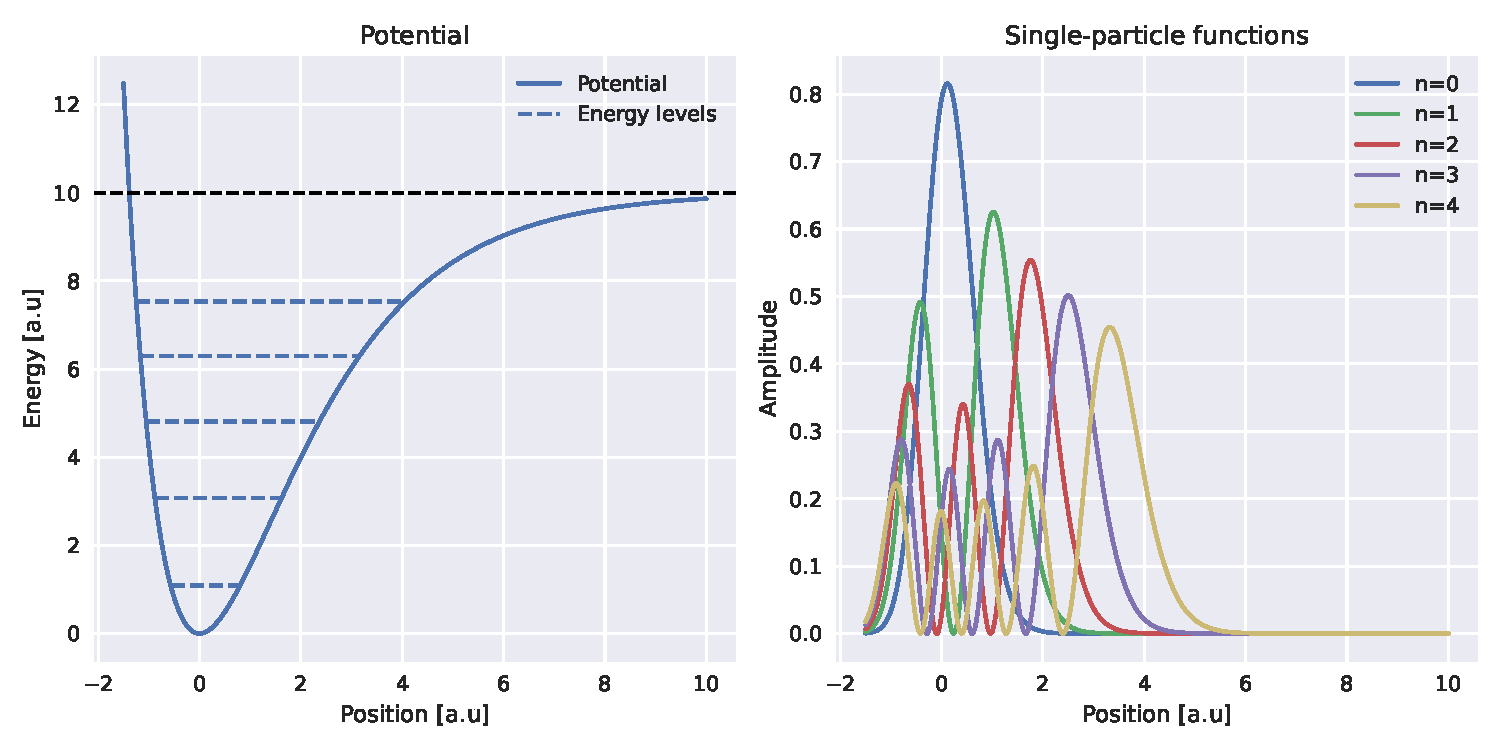
\includegraphics[width=0.8\textwidth]{figs/potential_spf.pdf}
    \caption{The Morse potential and the 5 lowest energy levels and energy eigenfunctions. The dissociation energy, $D$, is highlighted by the black dashed line. The parameters for this visualization of a Morse potential are $D=10, a=0.5, x_0=0$.}
    \label{fig:morse_potential}
\end{figure}
\textcolor{red}{TODO: Fix the figsize so text is correct size.}

%% Double well
\\ \\
Now, we would like to make a potential trap for \emph{two} separate particles, as our qubit system will be a two-particle system. To do so, we construct a double Morse potential well, simply by adding two Morse potentials together. We flip the right potential well, so that the minima are at the same position, and the potential is symmetric (given symmetric parameters). This gives us the double Morse potential as
\begin{equation}
    V(r) = D_L(e^{-c_L(r-r_{0,L})} - 1)^2 + D_R(e^{c_R(r-r_{0,R})} - 1)^2
\end{equation}
where the subscripts L and R correspond to left and right well, respectively. The parameter $D$ controls the depth of the potential well, whilst $c$ has some control over the width of the well, through the steepness of the exponential functions decay (and thus the curvature, and width, of the well). A smaller $c$ parameter constitues a wider well as the function would then decay slowly. The parameter $r_0$ is the position of the well minima. 

\begin{itemize}
    \item Presentation of the actual potential
    \item Why it is used, and where
    \item Connection to the long-range morse that is very popular
    \item Why we use it
    \item Form of the potential
    \item our construction of a double Morse potential well
    \item Some plots of the potential, and it's energy levels (show that they are quantized, but not equally spaced)
\end{itemize}

\section{Entanglement}
The concept of entanglement is a fundamental feature of quantum mechanical systems, distinguishing interacting quantum systems from classical systems. Conceptually introduced by Einstein, Podolski, and Rosen in their 1935 EPR paper \cite{EPR_1935}, the term \emph{entanglement} was later formalized by Schrödinger in the same year \cite{Schrödinger_1935}. Entanglement measures the correlations between two or more quantum mechanical subsystems. Any system with more than one degree of freedom exhibits such correlations between the "allowed states" in the system, and these correlations make the system non-separable. This means that, even if we have a complete description of the full system, we may not have a complete description of the correlated (entangled) subsystems. For a system of multiple particles, this implies that the state of each particle cannot be described independently of the states of the other particles, even if they are spatially separated by large distances. As Einstein famously expressed, there exists what he referred to as \emph{"spooky action at a distance"}, a phenomenon that classical physics fails to explain or replicate.\\ \\
\subsection*{Bell states}
In our system, we will be working in a bipartite system. This means that we have two subsystems, $L$ and $R$ (left and right), which are connected by a coupling Hamiltonian. Our two subsystems are two electrically charged particles, each trapped in a Morse potential well \textcolor{red}{ref til Morse potential bilde av systemet}, which then are coupled through the Coulomb interaction. 
To illustrate the concept of entanglement, we can consider a simple example of two distinguishable particles, $A$ and $B$, in a two-particle system, with two available states in each subsystem (ground state and excited state). The state of the system can be expressed as a product state, where each particle is in a separate state:
\begin{align*}
    \ket{\Psi} = \ket{\psi_A}\otimes\ket{\psi_B}
\end{align*}
where the available states are $\ket{\psi_A} = \ket{0} \text{or} \ket{1}$ and $\ket{\psi_B} = \ket{0} \text{or} \ket{1}$. The system can be in any of the four possible product states: 
\begin{align*}
    \ket{00} = \ket{0}_A\otimes\ket{0}_B, \quad \ket{01} = \ket{0}_A\otimes\ket{1}_B, \\
    \ket{10} = \ket{1}_A\otimes\ket{0}_B, \quad \ket{11} = \ket{1}_A\otimes\ket{1}_B
\end{align*}
However, due to the influence of the coupling Hamiltonian, the system can evolve into an entangled state, in which the state of the particles are mutually dependent. An example of such entangled states are the Bell states, which are maximally entangled states of two qubits. These states are given by
\begin{align*}
    \ket{\Phi^+} &= \frac{1}{\sqrt{2}}(\ket{00} + \ket{11}) \\
    \ket{\Phi^-} &= \frac{1}{\sqrt{2}}(\ket{00} - \ket{11}) \\
    \ket{\Psi^+} &= \frac{1}{\sqrt{2}}(\ket{01} + \ket{10}) \\
    \ket{\Psi^-} &= \frac{1}{\sqrt{2}}(\ket{01} - \ket{10})
\end{align*}
\\ 
In these states, measurements of the state of particle $A$ will immediately give information about the state in which particle $B$ is in, and vice versa. For example, if we prepare our systm in the Bell state $\ket{\Phi^+}$ and measure particle $A$ and find it in the state $\ket{0}$, we can immediately conclude that particle $B$ is also in the state $\ket{0}$. This is a fact, regardless of the physical separation of the two particles and was the basis for the EPR paradox \cite{EPR_1935}. This phenomenon, entanglement, is a direct consequence of the non-locality of quantum mechanics, and is a key resource for many quantum technologies, such as quantum computing, quantum cryptography, and quantum teleportation.\textcolor{red}{find sources}\\ 

\subsection*{Quantifying, and measuring entanglement}
While entanglement is conceptually well understood, quantifying it in physical systems - especially continuous and/or spatially extended systems like ours - requires precise mathematical tools. In our system of two charged particles confined in a double Morse well system (\textcolor{red}{Ref til Morse}), we aim to characterize the degree of entanglement between subsystems $L$ and $R$ that emerges due to the Coulomb coupling. To accomplish this, we shall turn to established entanglement measures such as the \emph{von Neumann entropy}, which will allow us to quantify the extent to which subsystms $L$ and $R$ are entangled. To do so, we will also introduce the concept of the reduced density matrix and explore it's physical intepretation in the context of our bipartite system.
\\ \\
In classical physics, we always assume the system to exists in well-defined, definite states, with any uncertainty arising solely from a \emph{lack of information or knowledge}. For example, a certain object will have a specific location in phase space, regardless of our knowledge of what this location is. This is what we call \emph{pure states}. States that give a complete and unambigous description of the system. In quantum mechanics the situation is more nuanced. While there are systems that can be described by such pure states (and represented by a single state vector), many systems require a more general description, particularly large entangled systems of subsystems. In such cases, while the entire system as a whole is in a well-defined quantum state, the smaller subsystems may not have definite states of their own. Instead they can exists in a \emph{mixed state}, which represents a statistical mixture - an ensamble - of different possible (pure) quantum states.
To summarize, a mixed state is a probabilistic combination of pure states, where the system is in one of the pure states with a certain probability. This is a direct consequence of the entanglement between the subsystems, as the correlations between them lead to uncertainty in the description of each subsystem. As opposed to the classical uncertainty, which arises from a lack of information, the uncertainty in quantum mechanics is a fundamental property of the system itself. This means that even if we have complete knowledge of the entire system, and it exists in a pure state, we may not be able to assign definite states to the subsystems meaning they are in mixed states. 
\\ \\ 
Thus describing these mixtures require a more general formalism, and to do so we introduce the \emph{density matrix formalism}. First introduced by John von Neumann in 1927\cite{neumann1927}, the density matrix formalism allows for expressing quantum states by both pure and mixed states and it's an essential tool for understanding and quantifying entanglement, since it encapsulates information about how a subsystem becomes "uncertain" due to its correlations with the rest of the system. As a representation of the \emph{density operator}, which the two terms in practice are used interchangeably, the density matrix (operator) is given as
\begin{equation}
    \rho = \sum_i w_i\ket{\psi_i}\bra{\psi_i}\label{eq:density_matrix}
\end{equation}
where the probability weight $w_i$ is the probability of finding the system in the pure state $\ket{\psi_i}$. The density matrix is a positive semi-definite operator, and it has the following properties:
\begin{itemize}
    \item $\text{Tr}(\rho) = 1$, meaning the trace of the density matrix is equal to 1, given that $\rho$ is a pure state. $\text{Tr}(\rho) < 1$ for mixed states.
    \item $\rho^\dagger = \rho$, meaning the density matrix is Hermitian.
    \item $\rho \geq 0$, meaning the density matrix is positive semi-definite.
\end{itemize}
Returning to our simple system of two distinguishable particles, we can express the density matrix of the system as
\begin{align*}
    \rho_{AB} = \begin{pmatrix}
        \rho_{00, 00} & \rho_{00, 01} & \rho_{00, 10} & \rho_{00, 11} \\
        \rho_{01, 00} & \rho_{01, 01} & \rho_{01, 10} & \rho_{01, 11} \\
        \rho_{10, 00} & \rho_{10, 01} & \rho_{10, 10} & \rho_{10, 11} \\
        \rho_{11, 00} & \rho_{11, 01} & \rho_{11, 10} & \rho_{11, 11}
    \end{pmatrix}
\end{align*}
where the diagonal elements of the density matrix are the probability populations of the system being in the corresponding states $\ket{00}, \ket{01}, \ket{10}, \ket{11}$, while the off-diagonal elements are the coherences between said states - signatures of superposition states. Such superposition states differ from mixed states, as they are not statistical mixtures of pure states, but rather linear combinations of pure states. But how do we measure the entanglement in our system? To do so, we've mentioned the von Neumann entropy, which is a measure of the amount of information that is missing from the system. The von Neumann entropy is defined as
\begin{equation}
    S(\rho) = -\text{Tr}(\rho \ln \rho)
\end{equation}
where $\rho$ is the density matrix of the system. But how do we relate this to entanglement when working with multiple entangled subsystems? We then need to find the \emph{reduced density matrix}, which is a partial trace of the full density matrix over the other subsystem. Effectively, this means we are tracing out (or removing) the degrees of freedom in the other subsystems, which do not directly contribute to the entanglement. The reduced density matrix for subsystem $A$ is given as
\begin{equation}
    \rho_A = \text{Tr}_B(\rho_{AB}) = \sum_{i}\bra{i_B}\rho_{AB}\ket{i_B}
\end{equation}
where $\ket{i_B}$ are the basis states of subsystem $B$. The reduced density matrix for subsystem $B$ is given in a similar manner. The von Neumann entropy of the reduced density matrix is then given as
\begin{equation}
    S(\rho_A) = -\text{Tr}(\rho_A \ln \rho_A)
\end{equation}
and it can easily be shown that $S(\rho_A) = S(\rho_B)$, meaning the entanglement is symmetric between the two subsystems, which is to be expected. 


\\\\ 
Another useful aspect of the density matrix formalism is that it naturally ties together with measurements in quantum mechanics. Let us consider a quantum system expressed by a density matrix $\rho$ as in \eqref{eq:density_matrix}, and we want to measure an observable $O$ in the system. The expectation value of the observable is given as
\begin{align*}
    \braket{O} = \sum_i w_i\bra{\psi_i}O\ket{\psi_i} = \sum_i w_i\text{Tr}\big(\ket{\psi_i}\bra{\psi_i}O\big) = \text{Tr}\big(\sum_i w_i \ket{\psi_i}\bra{\psi_i}O\big) = \text{Tr}(\rho O)
\end{align*}
and we see how powerful this notation is, we can quickly calculate expectation values of operators (observables) by a simple trace operation. 

\subsection*{Avoided crossings}
In our coupled, double well system \textcolor{red}{ref til morse potential}, the emergence of entanglement is a direct consequence of the Coulomb coupling between the two subsystems. This coupling will give rise to a phenomenon known as \emph{avoided crossings}\cite{nazir2005anticrossings}, regions in the parameter space where the energy levels of the two subsystems come close to each other, but do not cross due to the coupling of the two subsystems. This coupling makes it so that the energy levels that may be degenerate in the uncoupled system, are no longer degenerate in the coupled system and they are no longer independent, and the system is no longer separable or expressable as a product state. This means our two subsystems will be entangled, and the energy levels will be shifted due to the coupling and this we can use to manipulate the system. \\ \\
To illustrate this, we can consider a simple example of a two level system, with two energy levels $E_1$ and $E_2$, which are degenerate in the uncoupled system, i.e $E_1 = E_2$. Introducing a coupling term $V$, the effectiv Hamiltonian of the system can be expressed as
\begin{align*}
    H = \begin{pmatrix}
        E_1 & V \\
        V & E_2
    \end{pmatrix}
\end{align*}
where $V$ is the coupling strength between the two levels. The eigenvalues of this Hamiltonian are given as
\begin{align*}
    E_\pm = \frac{E_1 + E_2}{2} \pm \sqrt{\frac{(E_1 - E_2)^2}{4} + V^2}
\end{align*}
and we can see that the energy levels are shifted due to the coupling, and they will never cross for $V\neq0$. Consider now a dynamical system, where there is some explicit time-dependence in the Hamiltonian, with a constant coupling strength $V$.
\begin{align*}
    H(t) = \begin{pmatrix}
        E(t) & V \\
        V & -E(t)
    \end{pmatrix} = \begin{pmatrix}
        vt & V \\
        V & -vt
    \end{pmatrix}
\end{align*}
where $E(t)$ is the time-dependent energy level of the system, with $v$ the sweeping parameter, that sweep the energy levels towards each other (they are equal at $t=0$). Simulating for a time starting from $t<0$, where the energy levels are degenerate we will highlight the avoided crossing at $t=0$, and we get what is called a \emph{Landau-Zener transition} \cite{landau1932theorie, zener1932non}. 
\begin{figure}[h!]
    \centering
    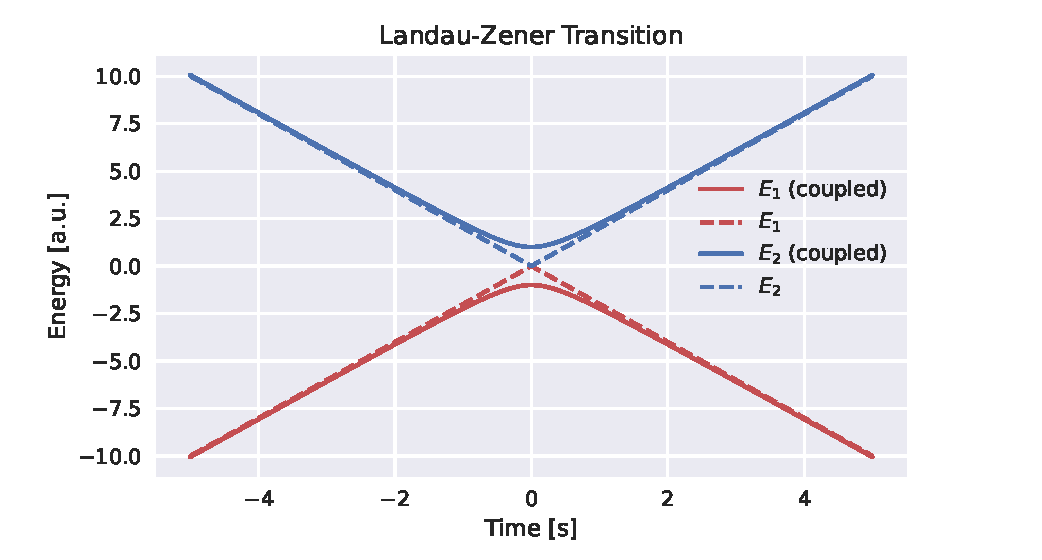
\includegraphics[width=0.8\textwidth]{figs/avoided_crossing.pdf}
    \caption{The avoided crossings in a two-level system as a function time $t$. The energy levels are shifted due to the coupling, and the energy levels do not cross, but rather "avoid" each other.}
    \label{fig:avoided_crossings}
\end{figure}
As we can see, the Coulomb coupling between the two subsystems results in the energy levels 'avoiding' eachother, while the non-interacting system would have crossed at $t=0$ (as indicated by the dotted lines). But what happens with the wavefunctions prepared in th system? Initializing the system in the ground state $\psi_0 = \ket{0}$, we shall see that what happens at the avoided crossing depends heavily on both coupling strength $V$ and sweeping paramter $k$, through the Landau-Zener formula \cite{landau1932theorie, zener1932non}:
\begin{align*}
    P_{0\rightarrow1} = e^{-\frac{2\pi V^2}{\hbar k}}
\end{align*}
which governs the probability of the system to transitions between the two energy levels. As visualized in the following plot \eqref{fig:landau_zener}, we can see how the sweeping parameter $k$ governs how the avoided crossing affect the prepared wavefunction, in one case we achive some minor level of mixing between the two basis states, while in the other case we achieve a full transition between the two states.
\begin{figure}[h!]
    \centering
    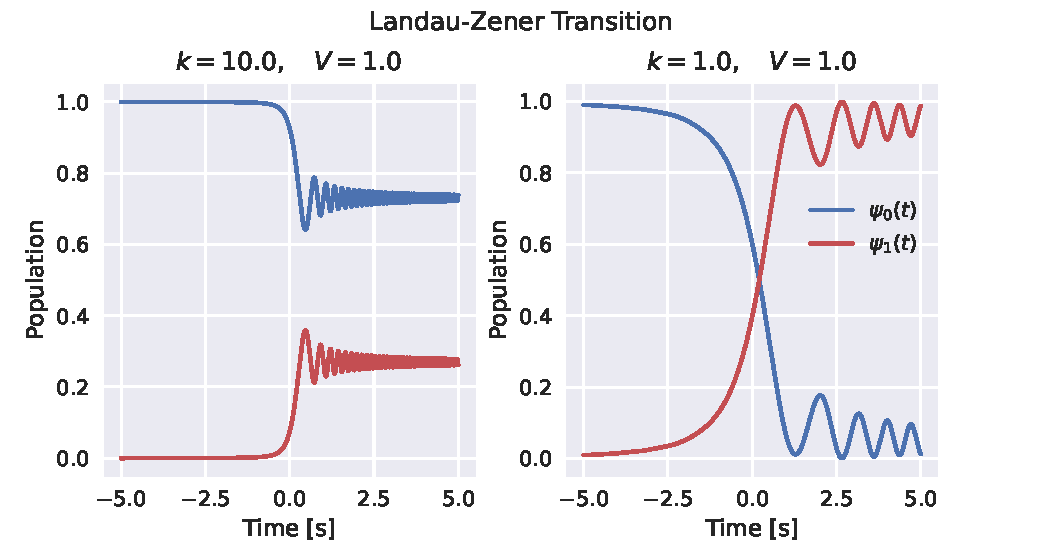
\includegraphics[width=0.8\textwidth]{figs/landau_zener.pdf}
    \caption{The Landau-Zener transition probability as a function of the coupling strength $V$ and the sweeping parameter $k$. The probability of the system to transition between the two energy levels is given by the Landau-Zener formula.}
    \label{fig:landau_zener}
\end{figure} 



\begin{itemize}
    \item What is entanglement
    \item Why is it important
    \item How do we measure it
    \item How do we create it
    \item How do we use it - avoided crossings, ref \cite{nazir2005anticrossings}
\end{itemize}



\section{Quantum time evolution}
In quantum mechanics, the time evolution of a quantum system is described by the Schrödinger equation\eqref{eq:tdse}. The TDSE shows the behaviour of a quantum system over time under the influence of the system Hamiltonian. While simple systems without time-dependence admit closed-form solutions, most physically realisable systems - especially those relevant for quantum control and information - exhibit time-dependent behaviour. Treating such systems that cannot be solved analytically, require numerical methods to approximate the systems evolution. Understanding time evolution is crucial for modelling driven systems such as qubit under external control field, where energy transitions reveal non-trivial dynamics\cite{landau1932theorie, zener1932non}, or simulating quantum gates in quantum computing \cite{leinonen2024coulomb, }.\textcolor{red}{trenger flere kilder og tilfeller}. In this section, we outline the framework for quantum time evolution and introduce the time-evolution operator, which is at the heart of quantum dynamics, and the basis for our numerical methods. We will also conceptualize the steps behind the numerical framework for solving the time-dependent Schrödinger equation, and also for discretizing the time evolution operator. \\
\subsection*{Time evolution operator}
Simulating the dynamics of any quantum system is seen through the evolution of the quantum mechanical state representing the system at hand. The time evolution of a quantum state from time $t_0$ to $t$ is expressed by the linear unitary time-evolution operator $U(t, t_0)$, which is a solution to the time-dependent Schrödinger equation.\cite{sakurai1986modern} This operator should do the following
\begin{equation}
    \ket{\Psi(t)} = U(t, t_0)\ket{\Psi(t_0)}
\end{equation}
and it must satisfy the following critera:
\begin{itemize}
    \item \textbf{Unitarity:} $U(t, t_0)U^\dagger(t, t_0) = U^\dagger(t, t_0)U(t, t_0) = \mathbb{1}$, meaning it preserves the norm of the quantum mechanical state.
    \item \textbf{Composition property:} $U(t_2, t_0) = U(t_2, t_1)U(t_1, t_0)$, meaning the time-evolution operator is a composition of smaller time-evolution operators that are time-ordered ($t_2>t_1>t_0$).
    \item \textbf{Continuity:} $\lim_{dt\to 0}U(t_0 + dt, t_0) = \mathcal{1}$, meaning the time-evolution operator is continuous, and reduces to identity when the time difference is zero.
\end{itemize}
All these critera can be satisfied by 
\begin{align*}
    U(t_0 + dt, t_0) = 1 - i\Omega(t_0) dt
\end{align*}
where $\Omega$ is a Hermitian operator, and $dt$ is the infinitesimal time difference. The 3rd criteria is satisfied naturally as $dt$ goes to zero, while the 1st and 2nd criteria is satisfied to first order 
\begin{align*}
    U^\dagger(t_0 + dt, t_0)U(t_0 + dt, t_0) = (1 + i\Omega(t_0)^\dagger)(1 - i\Omega(t_0)) = 1 + \mathcal{O}(dt^2) \approxeq 1
\end{align*}
and
\begin{align*}
    &U(t_0 + 2dt, t_0) = 1 - i2\Omega(t_0)dt, \\
    &U(t_0 + 2dt, t_0 +dt)U(t_0 + dt, t_0) = 1 - 2i\Omega(t_0)dt + \mathcal{O}(dt^2)
\end{align*}
if we have a small enough time-step $dt$, where we can safely ignore higher order terms. But how to identify the operator $\Omega$? We identify from classical mechanics that the Hamiltonian operator is the propagator of the system \cite{sakurai1986modern}, 
\begin{align*}
    \Omega = \frac{H}{\hbar}
\end{align*}
meaning, 
\begin{align*}
    U = 1 - \frac{i}{\hbar}Hdt
\end{align*}
which we can see is the first order approximation of the exponential series
\begin{align*}
    e^{\frac{-i}{\hbar}Ht} = 1 - \frac{i}{\hbar}Ht + \frac{1}{2!}\bigg(\frac{-i}{\hbar}Ht\bigg)^2 + ...
\end{align*}
which is the full form of the time-evolution operator, often coined time-propagator, and is given by
\begin{equation}
    U(t, t_0) = \mathcal{T}\text{exp}\bigg(\frac{-i}{\hbar}\int_{t_0}^t H(t')dt'\bigg)\label{eq:time_evolution_operator}
\end{equation}
where the integral must be time-ordered, and swapped with the Dyson series expansion should the Hamiltonian be time-dependent, and non-commutative at different times (see chapter 2.1.2 in \cite{sakurai1986modern}). For a time-independent Hamiltonian $H$, the time-evolution operator simplifies to 
\begin{align*}
    U(t, t_0) = e^{\frac{-i}{\hbar}H(t-t_0)}
\end{align*}
allowing for analytical propagation of the system. In contrast, the time-dependent case \eqref{eq:time_evolution_operator} requires numerical treatment to solve the integral, as the exponential cannot be solved analytically. 
\subsection{Numerical time propagation}
The time-propagator in \eqref{eq:time_evolution_operator} involves a time-ordered exponential, which generally cannot be solved analytically for a time-dependent Hamiltonian $H(t)$. Therefore, we must look to numerical methods to approximate and solve the integral. Choice of method is crucial, and it depends on accuracy, computational cost and stability. There are some other criteria to consider when developing, or choosing, a numerical method for time propagation. The method should preserve the norm of the wavefunction, and it should preserve the unitarity of the time-evolution operator. 
\\\\ 
To simulate quantum time evolution numerically, we start by discretizing time into smaller intervals (time steps) $\Delta t$. Doing so allows us to approximate the time-evolution operator as a product of smaller time-evolution operators, which can be solved iteratively (recall the composition property of the time-evolution operator). At each step then, the wavefunction is evolved by approximating the true time-evolution operator on the time interval $[t, t+\Delta t]$. \\ \\
The simplest approximative method is the \emph{Euler-Cromer} method, a first order method given by Taylor expansion of the time-evolution operator
\begin{align*}
    U(t + dt, t) = 1 - \frac{i}{\hbar}H(t)dt
\end{align*}
which leads to an explicit update of the wavefunction as 
\begin{align*}
    \ket{\Psi(t + dt)} = \bigg(1 - \frac{i}{\hbar}H(t)dt\bigg)\ket{\Psi(t)}
\end{align*}
which is a simple and fast, but inaccurate method. While this method is simple to implement and computationally inexpensive, it suffers from numerical instability and is not unitary nor norm-preserving. This means that the wavefunction will not be normalized after each time step, and the norm of the wavefunction will diverge over time, and we may obtain non-physical results should we want to evolve for longer timespans. \\ \\ 
To improve the accuracy and stability of the time-propagation, higher-order methods that are norm-preservign are preferred. One approach is to employ the matrix exponential of the Hamiltonian, which is unitary by construction. This ensures that the time-evolution remain physically meaningful, at the cost of computational efficiency due to the costlyness of matrix exponentiation. There are several methods to further approximate such matrix exponentials, such as


\begin{itemize}
    \item Time evolution of a quantum system
    \item Schrödinger equation
    \item Time evolution operator
    \item Different numerical integrators
    \item Trotter-Suzuki decomposition?
    \item How do we simulate time evolution
    \item Time evolution of a qubit system
\end{itemize}
\end{document}